%%%%%%%%%%%%%%%%%%%%%%%%%%%%%%%%%%%%%%%%%
% Jacobs Landscape Poster
% LaTeX Template
% Version 1.0 (29/03/13)
%
% Created by:
% Computational Physics and Biophysics Group, Jacobs University
% https://teamwork.jacobs-university.de:8443/confluence/display/CoPandBiG/LaTeX+Poster
% 
% Further modified by:
% Nathaniel Johnston (nathaniel@njohnston.ca)
%
% This template has been downloaded from:
% http://www.LaTeXTemplates.com
%
% License:
% CC BY-NC-SA 3.0 (http://creativecommons.org/licenses/by-nc-sa/3.0/)
%
%%%%%%%%%%%%%%%%%%%%%%%%%%%%%%%%%%%%%%%%%

%----------------------------------------------------------------------------------------
%	PACKAGES AND OTHER DOCUMENT CONFIGURATIONS
%----------------------------------------------------------------------------------------

\documentclass[final, 20 pt]{beamer}

\usepackage[size = a0, scale=1.2]{beamerposter} % Use the beamerposter package for laying out the poster
\usepackage{pdfpages}
\usepackage{amsmath,amsthm,amssymb}
\usepackage{tikz}
\usepackage{pstricks}
\usepackage{ragged2e}
\usepackage{mathrsfs}
\usepackage{microtype}
\usepackage{bbm}
\usepackage{graphicx, wrapfig, subcaption, setspace, booktabs}
\usepackage{tabularx}
\usepackage{listings}
\usepackage{xcolor}
\usepackage{longtable}
%\usepackage{titlesec}
\usepackage{url, lipsum}
\usepackage{hyperref,bookmark}
\usepackage[T1]{fontenc}
\usepackage{amssymb}
\usepackage{orcidlink}
\usepackage{tabularx}
\usepackage{listings}
\usepackage{xcolor}
\usepackage{longtable}
\usepackage{setspace}
\usepackage{float}
\usepackage{multirow}
\usepackage[ruled,linesnumbered]{algorithm2e}


\usetheme{confposter} % Use the confposter theme supplied with this template

\setbeamercolor{block title}{fg=ngreen,bg=white} % Colors of the block titles
\setbeamercolor{block body}{fg=black,bg=white} % Colors of the body of blocks
\setbeamercolor{block alerted title}{fg=white,bg=dblue!70} % Colors of the highlighted block titles
\setbeamercolor{block alerted body}{fg=black,bg=dblue!10} % Colors of the body of highlighted blocks
% Many more colors are available for use in beamerthemeconfposter.sty

%-----------------------------------------------------------
% Define the column widths and overall poster size
% To set effective sepwid, onecolwid and twocolwid values, first choose how many columns you want and how much separation you want between columns
% In this template, the separation width chosen is 0.024 of the paper width and a 4-column layout
% onecolwid should therefore be (1-(# of columns+1)*sepwid)/# of columns e.g. (1-(4+1)*0.024)/4 = 0.22
% Set twocolwid to be (2*onecolwid)+sepwid = 0.464
% Set threecolwid to be (3*onecolwid)+2*sepwid = 0.708

\newlength{\sepwid}
\newlength{\onecolwid}
\newlength{\twocolwid}
\newlength{\threecolwid}
\setlength{\paperwidth}{48in} % A0 width: 46.8in
\setlength{\paperheight}{36in} % A0 height: 33.1in
\setlength{\sepwid}{0.024\paperwidth} % Separation width (white space) between columns
\setlength{\onecolwid}{0.22\paperwidth} % Width of one column
\setlength{\twocolwid}{0.464\paperwidth} % Width of two columns
\setlength{\threecolwid}{0.708\paperwidth} % Width of three columns
\setlength{\topmargin}{-0.5in} % Reduce the top margin size
%-----------------------------------------------------------

\usepackage{graphicx}  % Required for including images

\usepackage{booktabs} % Top and bottom rules for tables

%----------------------------------------------------------------------------------------
%	TITLE SECTION 
%----------------------------------------------------------------------------------------

\title{CO\textsubscript{2} and Cost Impacts of a Transportation-microgrid with Electric Vehicle Charging Infrastructure: a case study in Southern California} % Poster title

\author{Luis Fernando Enriquez-Contreras, Matthew Barth, Sadrul Ula} % Author(s)

\institute{Department of Electrical and Computer Engineering  \\ University of California, Riverside} % Institution(s)

%----------------------------------------------------------------------------------------

\begin{document}

\addtobeamertemplate{block end}{}{\vspace*{2ex}} % White space under blocks
\addtobeamertemplate{block alerted end}{}{\vspace*{2ex}} % White space under highlighted (alert) blocks

\setlength{\belowcaptionskip}{2ex} % White space under figures
\setlength\belowdisplayshortskip{2ex} % White space under equations

\begin{frame}[t] % The whole poster is enclosed in one beamer frame

\begin{columns}[t] % The whole poster consists of three major columns, the second of which is split into two columns twice - the [t] option aligns each column's content to the top

\begin{column}{\sepwid}\end{column} % Empty spacer column

\begin{column}{\onecolwid} % The first column

%----------------------------------------------------------------------------------------
%	OBJECTIVES
%----------------------------------------------------------------------------------------

\begin{alertblock}{Purpose}

\begin{itemize}
	\item The goal is to see the accuracy of simulated microgrid models when applied to a real system
	\item This validation's main contribution is documenting the difficulties and challenges involved in transitioning from a simulated model to real-life implementation
	\item This paper focuses on the problems and outcomes of the microgrid's full-size components and describes how software is implemented in a full-scale microgrid
	\item The validation results are compared to the simulated model to analyze the differences and similarities between simulated and real-life data
\end{itemize}

\end{alertblock}

%----------------------------------------------------------------------------------------
%	INTRODUCTION
%----------------------------------------------------------------------------------------

\begin{block}{Abstract}
	As an important part of Intelligent Transportation Systems (ITS), this paper presents a case study at the University of California, Riverside (UCR) that evaluates the effectiveness of different transportation-based microgrid configurations in reducing both carbon dioxide (CO\textsubscript{2}) emissions and electricity costs. CO\textsubscript{2} emissions are calculated using high-resolution California Independent System Operator (CAISO) CO\textsubscript{2} emissions data to accurately assess the environmental impact of each setup. Electric costs were also compared to determine the financial savings potential for the consumer. The results demonstrate that a peak-shaving transportation-microgrid strategy can effectively reduce CO\textsubscript{2} emissions in the range of 24\% to 38\% and costs from \$27,000 to \$29,000 per year, even when considering the additional demand from 12 vehicles charging daily at the building. However, careful consideration should be given to battery sizing, as peak-shaving has diminishing returns. Doubling the battery size may only provide an additional savings of \$2,000 per year with a negligible reduction in emissions. This highlights the importance of optimizing battery capacity to maximize cost-effectiveness and environmental impact.
\end{block}

%------------------------------------------------

%\begin{figure}
%\includegraphics[width=0.8\linewidth]{placeholder.jpg}
%\caption{Figure caption}
%\end{figure}

%----------------------------------------------------------------------------------------

\end{column} % End of the first column

\begin{column}{\sepwid}\end{column} % Empty spacer column

\begin{column}{\twocolwid} % Begin a column which is two columns wide (column 2)

\begin{columns}[t,totalwidth=\twocolwid] % Split up the two columns wide column

\begin{column}{\onecolwid}\vspace{-.6in} % The first column within column 2 (column 2.1)

%----------------------------------------------------------------------------------------
%	Setup
%----------------------------------------------------------------------------------------

\begin{block}{Microgrid Architecture}
	\begin{figure}[!htb] 		
		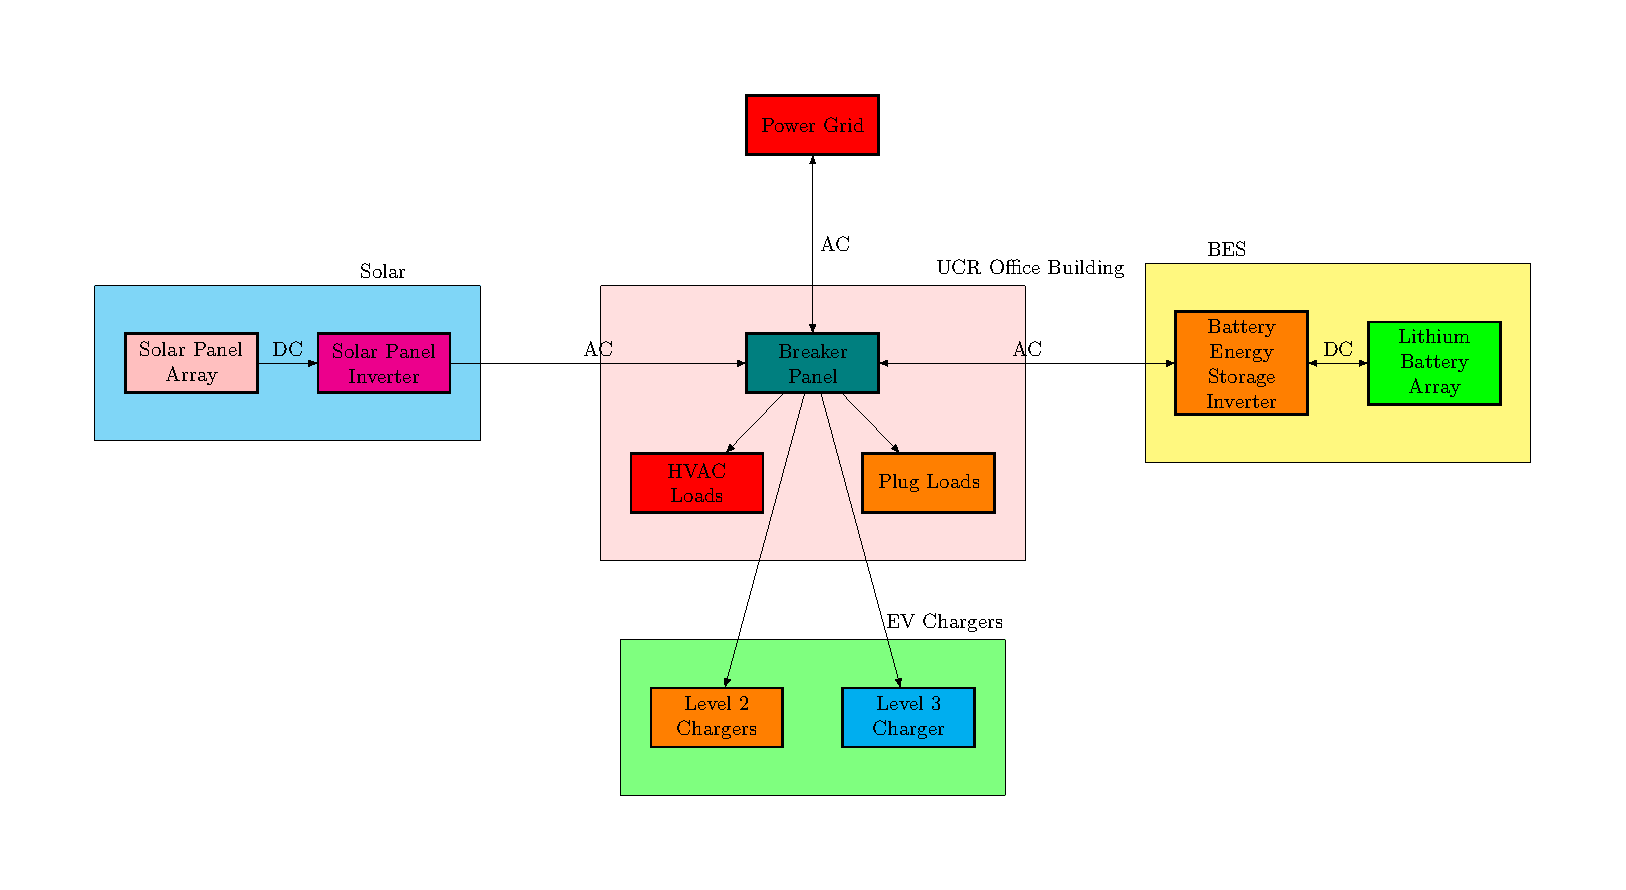
\includegraphics[width=\linewidth]{Fig/power_system_setup_modelica}
		\caption{\footnotesize Microgrid Architecture of our Case Study Example BESS: Battery Energy Storage System}
		\label{fig:powersystemsetupfull}
	\end{figure}
\end{block}

%----------------------------------------------------------------------------------------

\end{column} % End of column 2.1

\begin{column}{\onecolwid}\vspace{-.6in} % The second column within column 2 (column 2.2)

%----------------------------------------------------------------------------------------
%	METHODS
%----------------------------------------------------------------------------------------

\begin{block}{Control Software}

\begin{algorithm}[H]
	\caption{Microgrid Control Software}\label{alg:control_software}
	df $\gets$ dataset \\
	output $\gets$ [] \\
	count $\gets$ 0 \\
	delay $\gets$ 15 minutes \\
	new\_interval $\gets$ current\_time \\
	\While {data\_length $>$ count}
	{
		inverter\_power $\gets$ df.power[count]\\
		\While{new\_interval $>$ current\_time}
		{
			output $\gets$ inverter\_get\_data
		}
		count += 1 \\
		new\_interval += delay \\
	}	
\end{algorithm}

\end{block}

%----------------------------------------------------------------------------------------

\end{column} % End of column 2.2

\end{columns} % End of the split of column 2 - any content after this will now take up 2 columns width

%----------------------------------------------------------------------------------------
%	IMPORTANT RESULT
%----------------------------------------------------------------------------------------

%\begin{alertblock}{Important Result}
%
%Lorem ipsum dolor \textbf{sit amet}, consectetur adipiscing elit. Sed commodo molestie porta. Sed ultrices scelerisque sapien ac commodo. Donec ut volutpat elit.
%
%\end{alertblock} 

%----------------------------------------------------------------------------------------

\begin{columns}[t,totalwidth=\twocolwid] % Split up the two columns wide column again

\begin{column}{\onecolwid} % The first column within column 2 (column 2.1)

%----------------------------------------------------------------------------------------
%	MATHEMATICAL SECTION
%----------------------------------------------------------------------------------------

\begin{block}{EV Charging Simulations}
	\begin{figure}
		\centering
		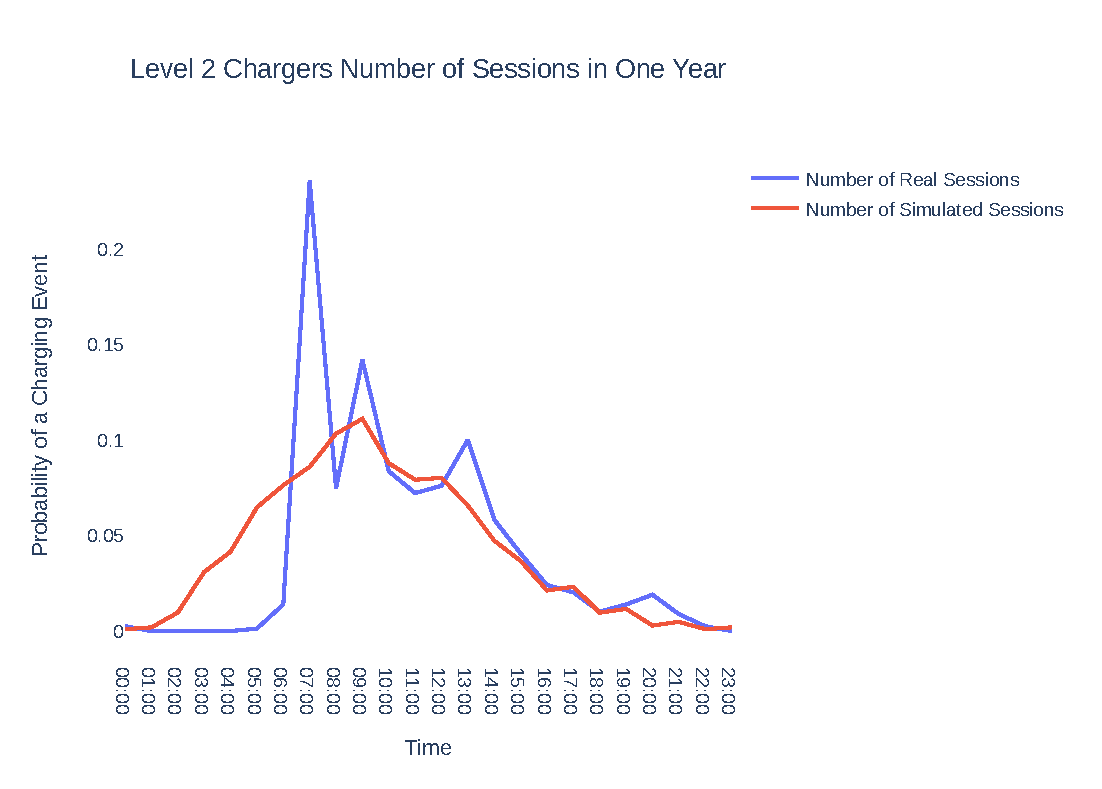
\includegraphics[width=\linewidth]{Fig/l2_avg_day_rand_poisson_1_hour_pdf}
		\caption{\footnotesize Validation of the Level 2 EV Charger Stochastic Process that Compares the Probability Density Function of Actual Charging Data to the Poisson Process}
		\label{fig:l2avgdayrandpoisson1hourpdf}
	\end{figure}

\end{block}

%----------------------------------------------------------------------------------------

\end{column} % End of column 2.1

\begin{column}{\onecolwid} % The second column within column 2 (column 2.2)

%----------------------------------------------------------------------------------------
%	RESULTS
%----------------------------------------------------------------------------------------

\begin{block}{Results}

	\begin{figure}[!htb]
			\centering
			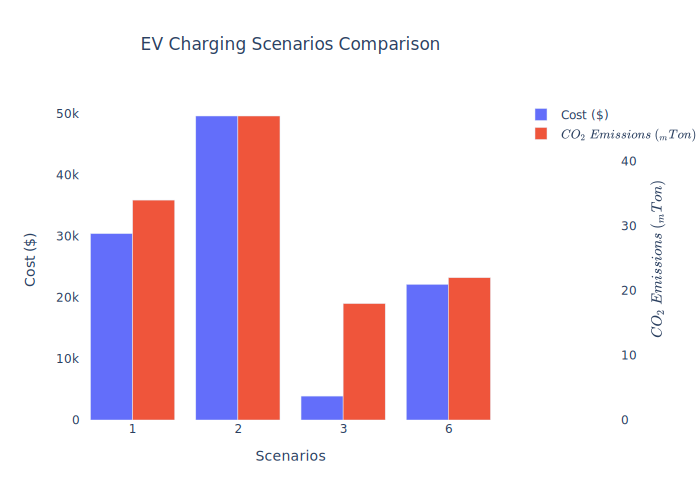
\includegraphics[width=\linewidth]{Fig/mg_scene_comparison}
			\caption{\footnotesize EV Charging Scenarios Comparison}
			\label{fig:mgscenecomparison}
	\end{figure}

\end{block}

%----------------------------------------------------------------------------------------

\end{column} % End of column 2.2

\end{columns} % End of the split of column 2

\end{column} % End of the second column

\begin{column}{\sepwid}\end{column} % Empty spacer column

\begin{column}{\onecolwid} % The third column

%----------------------------------------------------------------------------------------
%	CONCLUSION
%----------------------------------------------------------------------------------------
\begin{block}{}
		\begin{figure}[!htb] 		
		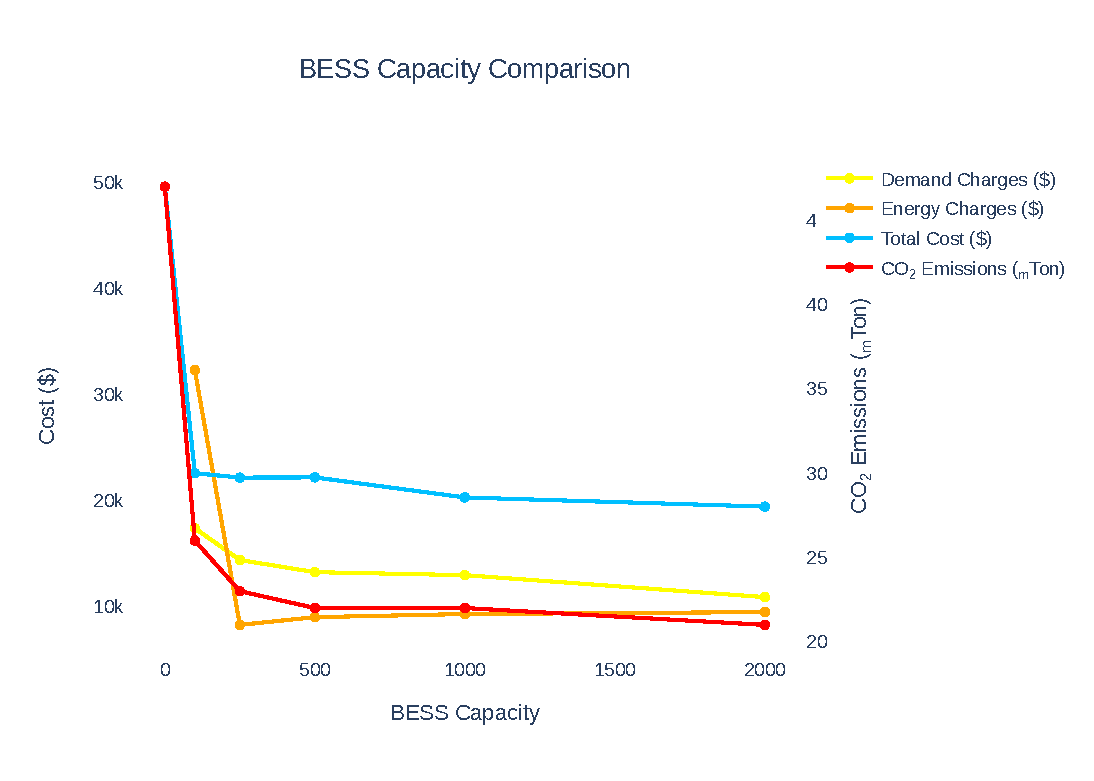
\includegraphics[width=0.85\linewidth]{Fig/bess_capacity_comparison}
		\caption{\footnotesize Cost and CO\textsubscript{2} Emissions for Different Battery Capacities}
		\label{fig:besscapacitycomparison}		
	\end{figure}
\end{block}

\begin{block}{Conclusion}

	\begin{itemize}	
		\item The results from this short validation demonstrate the possibility lowering the max demand of the net load, thus reducing the facility’s demand costs, by utilizing a BES system in combination with solar power
		\item The algorithm proposed and implemented achieved the goal of lowering the max demand, thereby reducing the stress on the grid
		\item Load prediction is needed to optimize data for the algorithm more accurately; optimization using shorter time intervals is also needed to reduce possible power surges
		\item This approach is unsuitable for islanding since the net load would exceed zero on multiple occasions
		\item Future improvements on this microgrid system will integrate load control, and a faster reaction time to the system that should enable full capability of automated islanding
	\end{itemize}

\end{block}

%----------------------------------------------------------------------------------------
%	ADDITIONAL INFORMATION
%----------------------------------------------------------------------------------------

%\begin{block}{Additional Information}
%
%Maecenas ultricies feugiat velit non mattis. Fusce tempus arcu id ligula varius dictum. 
%\begin{itemize}
%\item Curabitur pellentesque dignissim
%\item Eu facilisis est tempus quis
%\item Duis porta consequat lorem
%\end{itemize}
%
%\end{block}

%----------------------------------------------------------------------------------------
%	REFERENCES
%----------------------------------------------------------------------------------------

%\begin{block}{References}
%
%\nocite{*} % Insert publications even if they are not cited in the poster
%\small{\bibliographystyle{unsrt}
%\bibliography{sample}\vspace{0.75in}}
%
%\end{block}

%----------------------------------------------------------------------------------------
%	ACKNOWLEDGEMENTS
%----------------------------------------------------------------------------------------

\setbeamercolor{block title}{fg=red,bg=white} % Change the block title color

\begin{block}{Acknowledgements}

I would like to give a special thanks to the CE-CERT staff, and my family who have supported me throughout my research and without them this contribution would not be possible. \\

\end{block}

%----------------------------------------------------------------------------------------
%	CONTACT INFORMATION
%----------------------------------------------------------------------------------------

\setbeamercolor{block alerted title}{fg=black,bg=norange} % Change the alert block title colors
\setbeamercolor{block alerted body}{fg=black,bg=white} % Change the alert block body colors

\begin{alertblock}{Contact Information}

\begin{itemize}
\item Researcher: Luis Fernando Enriquez-Contreras
\item Web: \href{https://www.cert.ucr.edu/transportation-systems-vehicle-infrastructure-interaction}{https://www.cert.ucr.edu/transportation-systems-vehicle-infrastructure-interaction}
\item Email: \href{lenri001@ucr.edu}{lenri001@ucr.edu}
\item Phone: +1 (909) 763 1899
\end{itemize}

\end{alertblock}

\begin{center}
\begin{tabular}{ccc}
%\includegraphics[width=0.4\linewidth]{logo.png} & \hfill & %\includegraphics[width=0.4\linewidth]{logo.png}
\end{tabular}
\end{center}

%----------------------------------------------------------------------------------------

\end{column} % End of the third column

\end{columns} % End of all the columns in the poster

\end{frame} % End of the enclosing frame

\end{document}